\documentclass[11pt,a4paper,oneside]{article}

%------------------------------------------------------------
% PACKAGES
%------------------------------------------------------------
\usepackage[top=25mm, bottom=25mm, left=25mm, right=25mm,
            headheight=15pt]{geometry}
\usepackage{setspace}            % line spacing
\usepackage{mathptmx}            % Times New Roman (pdfLaTeX)
\usepackage[T1]{fontenc}
\usepackage[utf8]{inputenc}
\usepackage{graphicx}
\usepackage{float}
\usepackage{booktabs}            % professional tables
\usepackage{longtable}           % multi-page tables
\usepackage{multirow}
\usepackage{array}
\usepackage{tabularx}
\usepackage{amsmath}
\usepackage{amssymb}
\usepackage{bm}
\usepackage{caption}
\usepackage{subcaption}
\usepackage{xcolor}
\usepackage{pagecolor}
\usepackage{hyperref}
\usepackage{fancyhdr}
\usepackage{titlesec}
\usepackage{tocloft}
\usepackage{enumitem}
\usepackage{algorithm}
\usepackage{algpseudocode}
\usepackage{url}
\usepackage{afterpage}
\usepackage{emptypage}
\usepackage{microtype}
\usepackage{colortbl}
\usepackage[backend=biber,style=ieee]{biblatex}

\addbibresource{references.bib}

%------------------------------------------------------------
% SHORT TITLES FOR HEADER
%------------------------------------------------------------
\def\ProjectTitleShort{Reproducción de RBlockSim}
\def\DeptShort{Escuela Profesional de Ciencia de la Computación}

%------------------------------------------------------------
% COLOURS
%------------------------------------------------------------
\definecolor{dtunavy}{RGB}{0, 32, 91}
\definecolor{tablehead}{RGB}{0, 32, 91}
\definecolor{lightgray}{RGB}{245,245,245}

%------------------------------------------------------------
% LINE SPACING — 1.5
%------------------------------------------------------------
\onehalfspacing

%------------------------------------------------------------
% SECTION FORMAT
%------------------------------------------------------------
\titleformat{\section}
  {\bfseries\Large}
  {\thesection}
  {1em}
  {}

\titleformat{\subsection}
  {\bfseries\normalsize}
  {\thesubsection}
  {1em}
  {}

\titleformat{\subsubsection}
  {\itshape\normalsize}
  {\thesubsubsection}
  {1em}
  {}

%------------------------------------------------------------
% SPACING
%------------------------------------------------------------
\titlespacing*{\section}
  {0pt}
  {18pt}
  {12pt}

\titlespacing*{\subsection}
  {0pt}
  {12pt}
  {6pt}

\titlespacing*{\subsubsection}
  {0pt}
  {6pt}
  {3pt}

%------------------------------------------------------------
% CAPTION STYLE
%------------------------------------------------------------
\captionsetup[table]{position=above, labelfont=bf, font=small}
\captionsetup[figure]{position=below, labelfont=bf, font=small}

%------------------------------------------------------------
% HEADER/FOOTER
%------------------------------------------------------------
\pagestyle{fancy}
\fancyhf{}
\fancyhead[R]{\small\textit{\ProjectTitleShort}}
\fancyhead[L]{\small\textit{\DeptShort, UNSA}}
\fancyfoot[C]{\thepage}
\renewcommand{\headrulewidth}{0.4pt}

%============================================================
\begin{document}
%============================================================

\pagenumbering{roman}
\pagestyle{empty}

%============================================================
%  INNER TITLE PAGE
%============================================================
\def\myauthor{Alva Cornejo, Jose Javier}
\def\myteacher{Delgado Barra, Lucy Angela}
\def\mytitle{Reproducción de RBlockSim: Simulación Paralela y Distribuida para Blockchain}
\def\mycourse{REDES Y COMUNICACIÓN}
\def\myCUI{20230573}

\newgeometry{margin=1.5in}
\begin{titlepage}
	\centering
	{\huge{UNIVERSIDAD NACIONAL DE SAN AGUSTÍN} \par}
	\Large {\sc Facultad de Ingeniería de Producción y Servicios\\
	Escuela Profesional de Ciencia de la Computación}\\\vspace{0.5cm}
	
\includegraphics[width=0.65\textwidth]{unsa}\\\vspace{0.3cm}
    \LARGE\bf\mycourse\\\vspace{0.5cm}

	{\LARGE\bfseries \mytitle\par}
	\vspace{0.35cm}
	{\large\bfseries Informe de reproducción experimental\par}
	\vspace{1cm}
    {\Large {Docente:} \sc\myteacher}\\\vspace{0.5cm}
	{\Large {Estudiante:} \sc\myauthor\par \myCUI \par}

	\vfill

	{\Large Arequipa - Perú \par \today \par}
\end{titlepage}

\restoregeometry

%------------------------------------------------------------
% HYPERREF
%------------------------------------------------------------
\hypersetup{
  % colorlinks=true,
  linkcolor=dtunavy,
  citecolor=dtunavy,
  urlcolor=dtunavy,
  pdftitle={\mytitle},
}

%============================================================
%  MAIN TEXT
%============================================================
\cleardoublepage
\pagenumbering{arabic}
\setcounter{page}{1}

%============================================================
%  RESUMEN
%============================================================
\section*{Resumen}
\addcontentsline{toc}{section}{Resumen}

Este informe documenta la reproducción independiente de \emph{RBlockSim}, un simulador paralelo y distribuido de redes blockchain construido sobre el runtime de simulación de eventos discretos optimista ROOT-Sim. El trabajo se basa en el artefacto de reproducibilidad publicado por los autores y en el artículo presentado en SIGSIM-PADS 2025. La campaña experimental cubrió la validación estadística del modelo de Proof of Work (Figura~3 del artículo), los ataques del 51\,\% y de minería egoísta (Figuras~4 y~5), el rendimiento en tiempo de reloj (Figura~6), el uso máximo de memoria (Figura~7) y la evolución agregada de memoria (Figura~8). Se utilizaron únicamente los resultados de la carpeta \texttt{reproduced/*\_1}; la carpeta \texttt{*\_0} se descartó por corresponder a una ejecución incompleta.

Los resultados reproducidos confirman la validez estadística del modelo: la tasa de minería observada sigue a la esperada con $R^2 \ge 0.9969$ y un error absoluto medio (MAE) inferior a 0.013 en las tres redes evaluadas. El ataque del 51\,\% reproduce la diagonal esperada sin una aceptación desproporcionada de bloques, con MAE de 0.020--0.031. La minería egoísta reproduce las tendencias cualitativas del artículo: la tasa de éxito crece con la potencia de hash, se satura cerca de 1.0 para potencias altas y la profundidad 3 reduce el porcentaje de bloques del atacante en la cadena principal. Las curvas reproducidas son más irregulares que las del artículo porque se ejecutó una sola iteración por configuración, frente al promedio de cinco ejecuciones del artículo.

La reproducibilidad de rendimiento es solo parcial. La máquina disponible tenía 12 vCPU, por lo que las ejecuciones con 16, 22, 44, 66 y 88 hilos fallaron con el error \texttt{Demanding N cores, which are more than available (12)}. Solo son válidos los resultados con 1, 4 y 8 hilos. En ese rango, el artículo reporta speedups de hasta $4.45\times$ a 8 hilos para 10\,000 nodos, mientras que la reproducción obtiene $1.41\times$; en redes pequeñas (100 y 1\,000 nodos) la paralelización degrada fuertemente el tiempo, algo que el artículo también insinúa pero no con la magnitud observada. Los tiempos absolutos de un hilo son entre 4 y 25 veces menores que los del artículo, diferencia que no puede atribuirse únicamente al hardware y que se discute en el informe. El uso de memoria es consistente en orden de magnitud: 10\,000 nodos requieren 3.5--5.0\,GB (el artículo reporta aproximadamente 3.4--5.9\,GB) y 50\,000 nodos requieren 16.6--24.9\,GB; el artículo reporta 99.8\,GB para 100\,000 nodos en el texto, aunque su Figura~7 muestra valores cercanos a 35--47\,GB.

Se concluye que la reproducibilidad funcional y estadística de RBlockSim es alta, pero la reproducibilidad de rendimiento está fuertemente condicionada por el entorno de ejecución, el número de núcleos disponibles, el número de repeticiones y posibles diferencias de configuración no registradas en los metadatos.

\clearpage

%============================================================
%  1. INTRODUCCIÓN
%============================================================
\section{Introducción}

\subsection{Contexto y motivación}

Desde la aparición de Bitcoin en 2008 \cite{nakamoto2008bitcoin}, la tecnología blockchain se ha consolidado como una infraestructura para registrar transacciones de forma descentralizada, verificable e inmutable. Su adopción se ha extendido a criptomonedas, finanzas, trazabilidad de cadenas de suministro, identidad digital y sistemas de votación, entre otros dominios. La popularidad de la tecnología ha impulsado numerosas implementaciones que difieren en el algoritmo de consenso, el tamaño de bloque, el intervalo de generación, la topología de red y los mecanismos de propagación \cite{albshri2022simulators,paulavicius2021review}.

El diseño de una red blockchain exige decisiones que afectan propiedades emergentes como el rendimiento, la latencia, la escalabilidad, la eficiencia energética y la resistencia a ataques. Estas propiedades no pueden evaluarse con precisión mediante análisis estático, porque surgen de la interacción dinámica entre nodos, bloques, transacciones, retardos de red y comportamiento adversarial. La alternativa ideal sería desplegar la red a escala real; sin embargo, una red de decenas o cientos de miles de nodos requiere una cantidad prohibitiva de cómputo, memoria, almacenamiento y tiempo. La simulación ofrece un entorno controlado, reproducible y de bajo costo para observar esas propiedades emergentes \cite{pimpini2025rblocksim}.

La simulación secuencial de eventos discretos ha sido utilizada con éxito en simuladores de blockchain como BlockSim \cite{alharby2020blocksim,faria2019blocksim} y CBlockSim \cite{ma2022cblocksim}. No obstante, la simulación secuencial procesa los eventos uno a uno y está limitada por la memoria de una sola máquina, lo que restringe el tamaño de las redes que pueden estudiarse. La simulación paralela y distribuida de eventos discretos (PDES) permite distribuir los procesos lógicos entre varios núcleos o máquinas y reducir el tiempo de ejecución, a costa de introducir sincronización, rollbacks y nuevos retos de correctitud \cite{fujimoto1990pdes}.

RBlockSim \cite{pimpini2025rblocksim} es un banco de pruebas de alto rendimiento que combina un modelo modular de blockchain con el runtime optimista ROOT-Sim \cite{pellegrini2012rootsim}. El artículo original reporta validación estadística, resultados de ataques y resultados de rendimiento y memoria para redes de hasta 100\,000 nodos. La reproducibilidad de estos resultados es relevante porque permite verificar que las conclusiones no dependen de un entorno particular y porque documenta las condiciones bajo las cuales el rendimiento reportado puede alcanzarse.

\subsection{Objetivos}

Los objetivos específicos de este trabajo son:

\begin{enumerate}
  \item Reproducir la validación estadística del modelo de Proof of Work de RBlockSim (Figura~3 del artículo) y cuantificar la desviación respecto de la relación lineal esperada.
  \item Reproducir los experimentos de ataque del 51\,\% y de minería egoísta (Figuras~4 y~5) para las redes de 100, 1\,000 y 10\,000 nodos.
  \item Reproducir los experimentos de rendimiento en tiempo de reloj (Figura~6) para las redes y los números de hilos que el entorno permita ejecutar.
  \item Reproducir los experimentos de uso máximo de memoria (Figura~7) y de evolución agregada de memoria (Figura~8).
  \item Comparar los resultados reproducidos con los publicados, identificar discrepancias y documentar las limitaciones que impiden una comparación completa.
\end{enumerate}

\subsection{Alcance y organización}

La reproducción se realizó sobre el artefacto oficial de RBlockSim, utilizando una máquina con 12 vCPU y 31\,GiB de RAM. Por limitaciones de recursos, la red más grande de los experimentos de rendimiento y de la Figura~8 se redujo de 100\,000 a 50\,000 nodos, y no fue posible ejecutar los experimentos con 16 o más hilos. Además, se ejecutó una sola iteración por configuración, mientras que el artículo promedia cinco ejecuciones en la mayoría de los casos. Estas diferencias se detallan en la Sección~\ref{sec:metodologia} y se discuten en la Sección~\ref{sec:discusion}.

El resto del informe se organiza como sigue. La Sección~\ref{sec:marco} presenta el marco teórico de blockchain, PDES y RBlockSim. La Sección~\ref{sec:metodologia} describe el artefacto, la configuración experimental, el entorno y el procedimiento de análisis. La Sección~\ref{sec:resultados} presenta los resultados reproducidos. La Sección~\ref{sec:comparacion} compara los resultados con los del artículo. La Sección~\ref{sec:discusion} discute las implicancias y limitaciones. La Sección~\ref{sec:conclusiones} concluye y propone trabajo futuro.

%============================================================
%  2. MARCO TEÓRICO
%============================================================
\section{Marco teórico}
\label{sec:marco}

\subsection{Blockchain y Proof of Work}

Una blockchain es un libro contable distribuido que se replica entre los participantes de una red peer-to-peer. Las transacciones se agrupan en bloques; cada bloque contiene una referencia criptográfica al bloque anterior, un conjunto de transacciones, una marca de tiempo y un hash que lo identifica de forma única. La cadena de referencias hace que modificar un bloque invalide todos los bloques posteriores, lo que proporciona inmutabilidad y resistencia a la manipulación \cite{nakamoto2008bitcoin}.

En los sistemas basados en Proof of Work (PoW), los nodos denominados mineros compiten por resolver un problema criptográfico computacionalmente costoso. El primero en encontrar una solución válida propone el siguiente bloque y lo difunde a la red. Los demás nodos verifican la solución y el contenido antes de aceptar el bloque. La dificultad se ajusta para mantener un intervalo medio de bloque $\tau_b$ aproximadamente constante. La rama válida más larga se adopta como cadena principal; las ramas competidoras se denominan bifurcaciones o \emph{forks} \cite{gervais2016security}.

RBlockSim no ejecuta el cómputo criptográfico real, sino que modela el proceso de minería como un proceso de Poisson. Si el nodo $n$ posee una tasa de hash $H_n$ y la red tiene una tasa total $\sum_i H_i$, la probabilidad de que $n$ mine el siguiente bloque es proporcional a su participación:
\begin{equation}
  P(n \text{ mine}) = \frac{H_n}{\sum_i H_i}.
  \label{eq:prob}
\end{equation}
El tiempo hasta el siguiente bloque se muestrea de una distribución exponencial cuya media es
\begin{equation}
  \mathbb{E}[M_{\text{delay}}] = \tau_b \frac{\sum_i H_i}{H_n}.
  \label{eq:delay}
\end{equation}
Este modelo preserva la propiedad \emph{memoryless} de PoW y evita el costo computacional de resolver hashes reales \cite{pimpini2025rblocksim}.

\subsection{Simulación de eventos discretos y PDES}

En la simulación de eventos discretos, el estado del sistema cambia únicamente en instantes discretos asociados a eventos. Cada entidad simulada se representa mediante un proceso lógico (LP) con su propio estado y su propia cola de eventos. La simulación secuencial procesa los eventos en orden global de tiempo; la simulación paralela y distribuida (PDES) reparte los LPs entre varios ejecutores y debe garantizar que ningún evento se procese antes que sus dependencias causales \cite{fujimoto1990pdes}.

Existen dos familias principales de sincronización. La sincronización conservadora impide procesar un evento hasta tener la certeza de que no puede llegar uno anterior; es correcta por construcción, pero puede producir esperas ociosas \cite{chandy1981asynchronous}. La sincronización optimista, basada en el algoritmo Time Warp, permite procesar eventos de forma especulativa y corregir el estado mediante rollbacks cuando se detecta una violación de causalidad \cite{jefferson1985virtual}. El runtime mantiene un tiempo virtual global (GVT) que separa la parte segura de la parte especulativa de la simulación y coordina la recolección de estados y la cancelación de eventos \cite{jefferson2022virtual}.

El rendimiento de PDES depende de la relación entre el paralelismo disponible y el número de LPs, de la granularidad de los eventos, de la frecuencia de las dependencias y del costo de los rollbacks. Cuando hay pocos LPs por hilo, el sesgo de reloj y las cascadas de rollback pueden hacer que la ejecución paralela sea más lenta que la secuencial. Este fenómeno es especialmente relevante en redes pequeñas, donde cada nodo interactúa con muchos vecinos y genera una gran cantidad de eventos de propagación.

\subsection{RBlockSim}

RBlockSim es un simulador de blockchain construido sobre ROOT-Sim, un runtime PDES optimista de código abierto \cite{pellegrini2012rootsim}. Cada nodo de la red blockchain se modela como un LP. Los eventos principales son la generación de un bloque (\texttt{GENERATE\_BLOCK}), la recepción de un bloque (\texttt{RECEIVE\_BLOCK}) y la solicitud de un bloque padre que aún no se conoce (\texttt{REQUEST\_BLOCK}). El simulador mantiene una representación de la cadena organizada por niveles de altura, lo que permite acceso $O(1)$ a un nivel y un recorrido eficiente hacia atrás para cambiar de rama \cite{pimpini2025rblocksim}.

El módulo de red implementa una difusión por \emph{gossip}: cuando un nodo mina un bloque, lo envía a todos sus vecinos; cuando un nodo recibe un bloque por primera vez, selecciona un subconjunto aleatorio de sus vecinos de tamaño $\phi$ (fanout) y lo reenvía. La topología es un grafo simétrico generado aleatoriamente con un número mínimo y máximo de conexiones por nodo. Los retardos de propagación se muestrean de distribuciones exponenciales cuyas medias dependen de las regiones y de los anchos de banda configurados. La modularidad del simulador permite cambiar el consenso, la topología, el tamaño de bloque y el comportamiento adversarial sin reescribir el núcleo \cite{pimpini2025rblocksim}.

El artículo relaciona el número de eventos generados por bloque con el fanout y el número de vecinos. Si $p_i$ es el número de vecinos del nodo $i$ y $\phi$ es el fanout, el número de eventos de propagación por bloque es aproximadamente
\begin{equation}
  p_m + \sum_{i \ne m} \min(\phi, p_i),
  \label{eq:events}
\end{equation}
donde $m$ es el nodo que minó el bloque. Esta expresión explica por qué una topología densa o un fanout alto incrementan el costo de la simulación y el costo de los rollbacks \cite{pimpini2025rblocksim}.

\subsection{Ataques modelados}

RBlockSim implementa dos comportamientos maliciosos sobre una red Bitcoin con consenso de cadena más larga.

\textbf{Ataque del 51\,\%.} El atacante controla una fracción $h$ de la potencia de hash total y utiliza un parámetro de tolerancia al riesgo $c$. La tolerancia indica cuántos bloques está dispuesto a quedarse atrás respecto de una rama competidora si en la rama alternativa posee más bloques. Un atacante con suficiente potencia de hash puede intentar reescribir la cadena o revertir transacciones. El experimento mide el porcentaje de bloques de la cadena principal que fueron minados por el atacante; si el atacante no ejerce un comportamiento estratégico, ese porcentaje debe seguir aproximadamente la diagonal $y=h$.

\textbf{Minería egoísta.} El atacante oculta los bloques que mina y los libera selectivamente para intentar que los mineros honestos desperdicien trabajo y adopten la rama del atacante. El comportamiento se controla con la tolerancia al riesgo $c$ y la profundidad del ataque $d$, que indica cuántos bloques se minan en secreto antes de liberarlos. El experimento mide dos cantidades: el porcentaje de bloques del atacante que terminan en la cadena principal y la tasa de éxito del ataque, definida como la fracción de intentos de ocultamiento que consiguen que la red adopte la rama del atacante \cite{eyal2014majority,pimpini2025rblocksim}.

\subsection{Métricas de evaluación}

Para la validación estadística se comparan la tasa de minería observada $y_i$ con la tasa de hash esperada $x_i$ para cada nivel de potencia. Se utilizan el coeficiente de determinación
\begin{equation}
  R^2 = 1 - \frac{\sum_i (y_i-x_i)^2}{\sum_i (y_i-\bar{y})^2},
  \label{eq:r2}
\end{equation}
el error absoluto medio
\begin{equation}
  \mathrm{MAE} = \frac{1}{n}\sum_{i=1}^{n}|y_i-x_i|,
  \label{eq:mae}
\end{equation}
y la raíz del error cuadrático medio
\begin{equation}
  \mathrm{RMSE} = \sqrt{\frac{1}{n}\sum_{i=1}^{n}(y_i-x_i)^2}.
  \label{eq:rmse}
\end{equation}

Para los ataques se reporta el porcentaje de bloques del atacante en la cadena principal y la tasa de éxito. Para el rendimiento se reporta el tiempo de reloj en segundos, la memoria máxima en gigabytes y el speedup
\begin{equation}
  S(p) = \frac{T(1)}{T(p)},
  \label{eq:speedup}
\end{equation}
donde $T(p)$ es el tiempo de ejecución con $p$ hilos de trabajo. Un speedup mayor que 1 indica una mejora; un valor menor que 1 indica una degradación.

%============================================================
%  3. METODOLOGÍA
%============================================================
\section{Metodología de reproducción}
\label{sec:metodologia}

\subsection{Artefacto y flujo de ejecución}

La reproducción se realizó sobre el repositorio oficial \texttt{RBlockSim\_Reproducibility}, disponible en \url{https://github.com/AdrianoPi/RBlockSim_Reproducibility}. El artefacto está containerizado con Docker y organiza la campaña en tres bloques: ataques (Figuras~3, 4 y~5), rendimiento (Figuras~6 y~7) y Figura~8. El script \texttt{reproduce.sh} construye la imagen y ejecuta \texttt{entrypoint.py}, que a su vez invoca \texttt{repro\_runner.py} para lanzar las simulaciones y \texttt{repro\_plotter.py} para generar las figuras.

El flujo es el siguiente: (i) se genera una topología aleatoria con \texttt{generate\_topology.py}; (ii) se compila el ejecutable \texttt{rblocksim} con la topología y la configuración seleccionadas; (iii) se ejecutan las configuraciones de ataque o de rendimiento; (iv) los resultados se copian a \texttt{reproduced/results\_*\_N}; y (v) el trazador genera las figuras en \texttt{reproduced/plots/plots\_N}. Cada ejecución deja un archivo \texttt{out\_*.txt} con el tiempo de simulación, un archivo \texttt{err\_*.txt} con la configuración de ROOT-Sim y, en los experimentos de ataque, una carpeta \texttt{Results\_*} con las estadísticas por nodo y la información del ataque.

\subsection{Configuración experimental}

La configuración utilizada se muestra en la Tabla~\ref{tab:config}. Se ejecutó el artefacto completo con \texttt{what\_to\_reproduce = "all"}. Para los ataques se usaron 8 hilos de trabajo, tres tamaños de red (100, 1\,000 y 10\,000 nodos), un intervalo de bloque de 600\,s y una duración simulada de 24\,h. Para cada tamaño se probaron 20 potencias de hash del atacante, desde 0.01 hasta 0.99 en pasos de 0.05, dos tolerancias (1 y 2) para el ataque del 51\,\%, y dos tolerancias y tres profundidades (1, 2 y 3) para la minería egoísta. En total, cada tamaño de red comprende 160 ejecuciones: 40 del ataque del 51\,\% y 120 de minería egoísta.

Para el rendimiento se usaron cuatro tamaños de red (100, 1\,000, 10\,000 y 50\,000 nodos), dos intervalos de bloque (13\,s y 600\,s) y ocho números de hilos (1, 4, 8, 16, 22, 44, 66 y 88). La red de 50\,000 nodos sustituye a la red de 100\,000 nodos del artículo por limitaciones de memoria y tiempo. La Figura~8 se reprodujo con redes de 1\,000, 10\,000 y 50\,000 nodos, 8 hilos, intervalo de bloque de 600\,s, potencia de hash del atacante 0.4, tolerancia 2 y profundidad 2.

\begin{table}[H]
\caption{Configuración de los experimentos reproducidos.}
\label{tab:config}
\centering
\small
\renewcommand{\arraystretch}{1.15}
\begin{tabularx}{\textwidth}{lX}
\toprule
\rowcolor{tablehead}
\textcolor{white}{\textbf{Parámetro}} &
\textcolor{white}{\textbf{Valor}} \\
\midrule
Modo de reproducción & \texttt{all} (ataques, rendimiento y Figura~8) \\
Hilos en ataques & 8 \\
Redes en ataques & 100, 1\,000 y 10\,000 nodos \\
Potencia de hash del atacante & 0.01 a 0.99, paso 0.05 (20 valores) \\
Tolerancias (51\,\%) & 1 y 2 \\
Tolerancias y profundidades (egoísta) & $c \in \{1,2\}$, $d \in \{1,2,3\}$ \\
Intervalo de bloque en ataques & 600\,s \\
Duración simulada & 24\,h (86\,400\,s) \\
Redes en rendimiento & 100, 1\,000, 10\,000 y 50\,000 nodos \\
Intervalos de bloque en rendimiento & 13\,s y 600\,s \\
Hilos en rendimiento & 1, 4, 8, 16, 22, 44, 66 y 88 \\
Redes en Figura~8 & 1\,000, 10\,000 y 50\,000 nodos \\
Hilos en Figura~8 & 8 \\
Iteraciones por configuración & 1 \\
\bottomrule
\end{tabularx}
\end{table}

\subsection{Entorno de ejecución}

La Tabla~\ref{tab:entorno} compara el entorno del artículo con el utilizado en esta reproducción. El artículo ejecutó los experimentos en un servidor con dos procesadores Intel Xeon E5-2696 v4 de 2.20\,GHz, 22 núcleos físicos por procesador (44 núcleos físicos y 88 hyperthreads) y 256\,GB de RAM, sobre Ubuntu 22.04.5. La reproducción se ejecutó en un equipo con un procesador Intel Core i7-10850H de 2.70\,GHz, 6 núcleos físicos y 12 hyperthreads, 31\,GiB de RAM y Linux. La diferencia de recursos es el factor más importante para interpretar los resultados de rendimiento.

\begin{table}[H]
\caption{Comparación de los entornos de ejecución.}
\label{tab:entorno}
\centering
\small
\renewcommand{\arraystretch}{1.15}
\begin{tabularx}{\textwidth}{lXX}
\toprule
\rowcolor{tablehead}
\textcolor{white}{\textbf{Aspecto}} &
\textcolor{white}{\textbf{Artículo}} &
\textcolor{white}{\textbf{Reproducción}} \\
\midrule
Procesador & 2 $\times$ Intel Xeon E5-2696 v4 @ 2.20\,GHz & Intel Core i7-10850H @ 2.70\,GHz \\
Núcleos físicos & 44 (22 por socket) & 6 \\
Hyperthreads & 88 & 12 \\
Memoria & 256\,GB & 31\,GiB \\
Sistema operativo & Ubuntu 22.04.5 LTS & Linux (contenedor Docker) \\
Iteraciones & 5 (promedio) & 1 \\
Red más grande & 100\,000 nodos & 50\,000 nodos \\
\bottomrule
\end{tabularx}
\end{table}

\subsection{Selección y depuración de datos}

El artefacto genera una carpeta \texttt{reproduced/*\_N} por cada ejecución completa. En este trabajo se utilizó exclusivamente \texttt{reproduced/results\_attacks\_1}, \texttt{reproduced/results\_performance\_1} y \texttt{reproduced/results\_figure\_8\_1}. La carpeta \texttt{*\_0} corresponde a una ejecución previa incompleta y se excluyó para evitar mezclar datos de campañas distintas.

Las ejecuciones de rendimiento con 16, 22, 44, 66 y 88 hilos no llegaron a iniciar porque la máquina solo dispone de 12 unidades de cómputo. El error reportado por ROOT-Sim fue \texttt{Demanding N cores, which are more than available (12)}. En consecuencia, los únicos tiempos válidos son los de 1, 4 y 8 hilos. Los archivos \texttt{RAM\_usage\_peaks\_Bytes\_*.json} de las configuraciones fallidas contienen valores residuales del orden de $10^{-3}$\,GB; esos valores se excluyeron del análisis y de las figuras.

El trazador original de RBlockSim no filtra las ejecuciones fallidas: al no encontrar la línea de tiempo, asigna un tiempo de cero y dibuja un punto en cero. Por esa razón, las Figuras~6 y~7 generadas directamente por el artefacto no son utilizables para los números de hilos fallidos. En este informe se regeneraron ambas figuras usando únicamente los pares (tamaño de red, intervalo de bloque, hilos) que finalizaron correctamente. Las Figuras~3, 4, 5 y~8 no presentan este problema y se regeneraron a partir de los JSON procesados por el artefacto, con etiquetas en español y un estilo uniforme.

\subsection{Procedimiento de análisis}

Para la Figura~3 se agregaron todas las ejecuciones de ataque de cada tamaño de red. Para cada potencia de hash se promedió la tasa de minería observada sobre las ocho configuraciones de ataque (dos tolerancias del 51\,\% y seis combinaciones de tolerancia y profundidad de minería egoísta). Luego se calcularon $R^2$, MAE y RMSE respecto de la identidad.

Para las Figuras~4 y~5 se reconstruyeron las curvas a partir de las estadísticas por nodo. El porcentaje de bloques del atacante en la cadena principal se calculó como el cociente entre los bloques del atacante y la altura de la cadena principal, usando el par más frecuente entre todos los nodos para reducir el efecto de estados transitorios. La tasa de éxito de la minería egoísta se calculó con la misma definición operativa del trazador original: bloques del atacante normalizados por $d \cdot N$, divididos por el número de intentos de ocultamiento (exitosos más fallidos).

Para el rendimiento se extrajo el tiempo de la línea \texttt{Simulation completed in ... seconds} de cada archivo de salida. La memoria máxima se tomó del JSON de picos de RAM. El speedup se calculó con la Ecuación~\eqref{eq:speedup}. Los valores del artículo para las Figuras~6 y~7 se digitalizaron a partir del PDF y se contrastaron visualmente con las curvas publicadas; se usan como referencia aproximada y se identifican como tales en las tablas.

%============================================================
%  4. RESULTADOS
%============================================================
\section{Resultados de la reproducción}
\label{sec:resultados}

\subsection{Validación estadística}

La Figura~\ref{fig:validacion} muestra la tasa de minería observada frente a la tasa de hash esperada para las tres redes. En los tres casos la curva observada sigue de cerca la diagonal. La Tabla~\ref{tab:validacion} resume las métricas: $R^2$ entre 0.9969 y 0.9989, MAE entre 0.0086 y 0.0127 y RMSE entre 0.0095 y 0.0159. La red de 1\,000 nodos presenta el mejor ajuste; la de 10\,000 nodos muestra las mayores desviaciones, especialmente en potencias intermedias, aunque sin un sesgo sistemático apreciable.

\begin{table}[H]
\caption{Métricas de validación estadística de la Figura~3 reproducida.}
\label{tab:validacion}
\centering
\small
\renewcommand{\arraystretch}{1.15}
\begin{tabular}{lccc}
\toprule
\rowcolor{tablehead}
\textcolor{white}{\textbf{Nodos}} &
\textcolor{white}{\textbf{$R^2$}} &
\textcolor{white}{\textbf{MAE}} &
\textcolor{white}{\textbf{RMSE}} \\
\midrule
100    & 0.9982 & 0.0096 & 0.0122 \\
1\,000 & 0.9989 & 0.0086 & 0.0095 \\
10\,000 & 0.9969 & 0.0127 & 0.0159 \\
\bottomrule
\end{tabular}
\end{table}

\begin{figure}[H]
  \centering
  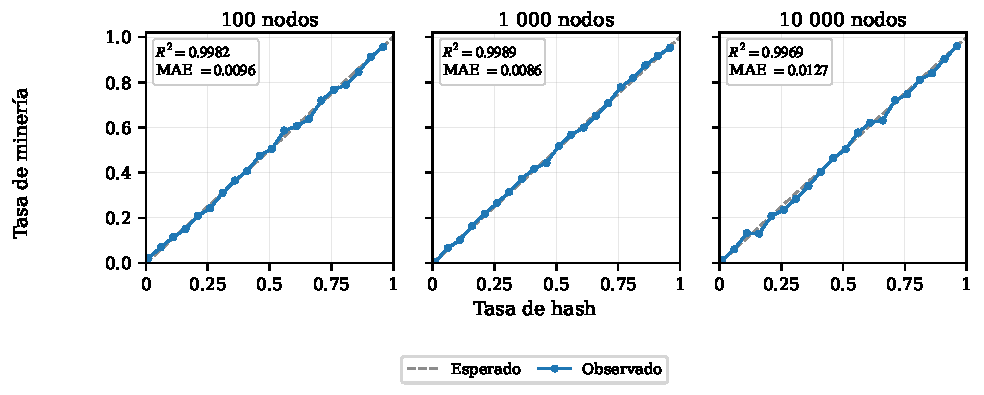
\includegraphics[width=\textwidth]{figures/fig_validacion.pdf}
  \caption{Validación estadística reproducida (equivalente a la Figura~3 del artículo). La línea gris punteada es la relación esperada $y=x$; la línea azul es la tasa de minería observada. Cada panel corresponde a un tamaño de red.}
  \label{fig:validacion}
\end{figure}

La cercanía a la diagonal confirma que el generador de bloques de RBlockSim respeta la proporcionalidad entre potencia de hash y tasa de minería. Las pequeñas diferencias son compatibles con el ruido estadístico de una sola ejecución por configuración y con el número finito de bloques minados en 24\,h (del orden de 6\,500 para un intervalo de 13\,s y de 145 para 600\,s).

\subsection{Ataque del 51\,\%}

La Figura~\ref{fig:51} muestra el porcentaje de bloques del atacante en la cadena principal frente a su potencia de hash, para las tolerancias 1 y 2. Las curvas siguen la diagonal esperada en los tres tamaños de red. No se observa una aceptación desproporcionada de bloques del atacante: para $h<0.5$ el porcentaje se mantiene por debajo o cerca de $h$, y para $h>0.5$ acompaña el crecimiento esperado. Las dos tolerancias producen curvas muy próximas entre sí, lo que sugiere que, en este escenario, la tolerancia al riesgo no altera de forma sustancial el resultado agregado.

\begin{figure}[H]
  \centering
  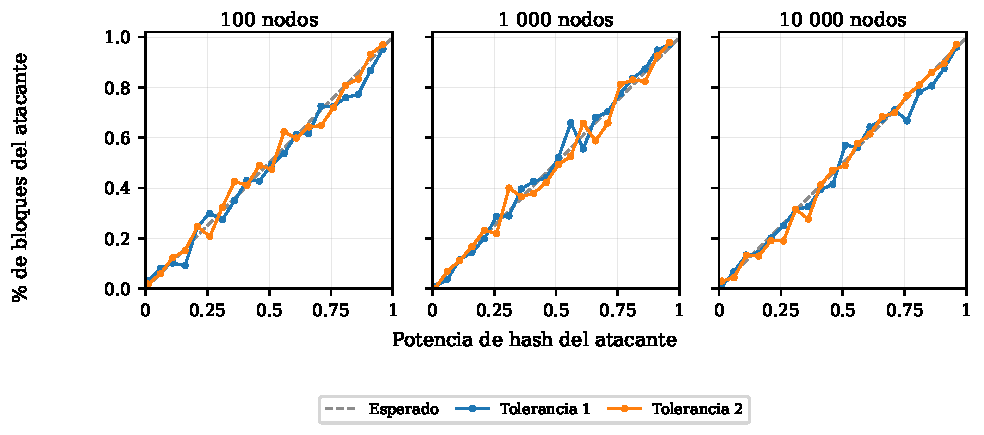
\includegraphics[width=\textwidth]{figures/fig_51.pdf}
  \caption{Ataque del 51\,\% reproducido (equivalente a las Figuras~4a--4c del artículo). Se muestra el porcentaje de bloques del atacante en la cadena principal frente a su potencia de hash, para las tolerancias 1 y 2. La línea gris punteada es la relación esperada $y=x$.}
  \label{fig:51}
\end{figure}

La Tabla~\ref{tab:51} cuantifica la desviación respecto de la diagonal. El MAE se sitúa entre 0.0197 y 0.0312, el error máximo entre 0.0667 y 0.0994 y el sesgo medio entre $-0.0152$ y $+0.0083$. El sesgo negativo más alto corresponde a 100 nodos con tolerancia 1; el sesgo positivo más alto corresponde a 1\,000 nodos con tolerancia 1. En todos los casos el error es inferior a 10 puntos porcentuales, un valor razonable para una sola realización por punto.

\begin{table}[H]
\caption{Error del ataque del 51\,\% respecto de la diagonal esperada.}
\label{tab:51}
\centering
\small
\renewcommand{\arraystretch}{1.15}
\begin{tabular}{lcccc}
\toprule
\rowcolor{tablehead}
\textcolor{white}{\textbf{Nodos}} &
\textcolor{white}{\textbf{Tol.}} &
\textcolor{white}{\textbf{MAE}} &
\textcolor{white}{\textbf{Error máx.}} &
\textcolor{white}{\textbf{Sesgo medio}} \\
\midrule
100    & 1 & 0.0312 & 0.0873 & $-0.0152$ \\
100    & 2 & 0.0259 & 0.0667 & $+0.0004$ \\
1\,000 & 1 & 0.0237 & 0.0994 & $+0.0083$ \\
1\,000 & 2 & 0.0310 & 0.0900 & $-0.0022$ \\
10\,000 & 1 & 0.0246 & 0.0933 & $-0.0101$ \\
10\,000 & 2 & 0.0197 & 0.0834 & $-0.0070$ \\
\bottomrule
\end{tabular}
\end{table}

\subsection{Minería egoísta}

La Figura~\ref{fig:selfish} muestra el porcentaje de bloques del atacante en la cadena principal para las seis combinaciones de tolerancia y profundidad. La Figura~\ref{fig:success} muestra la tasa de éxito del ataque. En ambos casos se observa el comportamiento cualitativo reportado por el artículo: a mayor potencia de hash, mayor éxito; la tasa de éxito es baja para $h<0.2$, crece de forma marcada entre 0.2 y 0.6 y se satura cerca de 1.0 para $h>0.8$.

\begin{figure}[H]
  \centering
  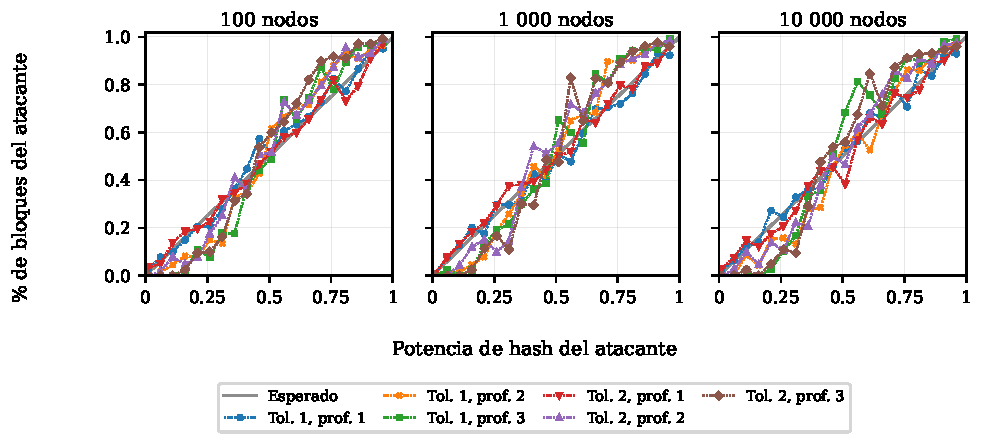
\includegraphics[width=\textwidth]{figures/fig_selfish_committed.pdf}
  \caption{Minería egoísta reproducida (equivalente a las Figuras~4d--4f del artículo). Porcentaje de bloques del atacante en la cadena principal frente a su potencia de hash, para dos tolerancias y tres profundidades. La línea gris es la relación esperada $y=x$.}
  \label{fig:selfish}
\end{figure}

\begin{figure}[H]
  \centering
  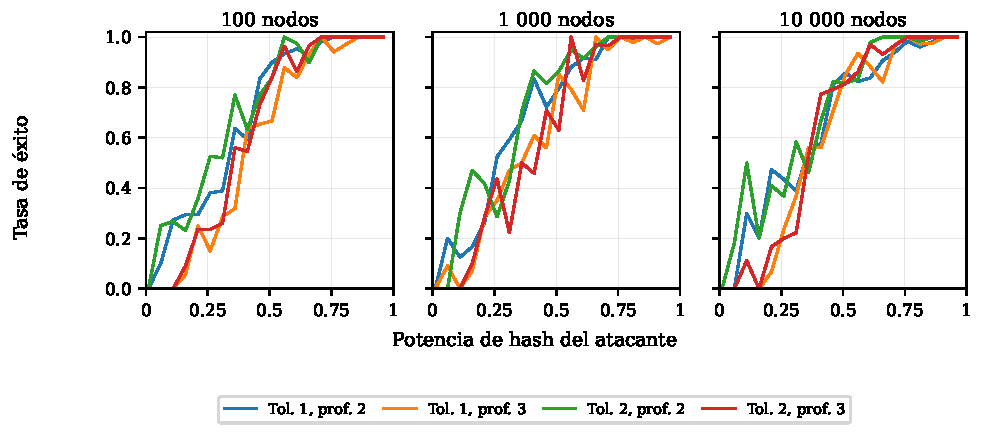
\includegraphics[width=\textwidth]{figures/fig_selfish_success.pdf}
  \caption{Tasa de éxito de la minería egoísta reproducida (equivalente a la Figura~5 del artículo). Cada panel corresponde a un tamaño de red; las curvas corresponden a las combinaciones de tolerancia y profundidad indicadas.}
  \label{fig:success}
\end{figure}

La Tabla~\ref{tab:selfish} resume el MAE del porcentaje comprometido. La profundidad 1 es la que mejor sigue la diagonal, con MAE de 0.024--0.032. La profundidad 2 duplica aproximadamente el error (0.062--0.081), y la profundidad 3 lo eleva a 0.084--0.103. En las tres redes, las curvas de profundidad 3 se sitúan por debajo de la diagonal para potencias bajas y medias, lo que indica que el atacante compromete menos bloques de los que le corresponderían por su potencia de hash. Este resultado es consistente con la observación del artículo de que atacar sin controlar al menos el 50\,\% de la potencia de hash es contraproducente en términos de bloques comprometidos en la cadena principal.

\begin{table}[H]
\caption{MAE del porcentaje de bloques comprometidos en minería egoísta.}
\label{tab:selfish}
\centering
\small
\renewcommand{\arraystretch}{1.15}
\begin{tabular}{lccccc}
\toprule
\rowcolor{tablehead}
\textbf{Nodos} & \textbf{Tol.} &
\textbf{Prof. 1} & \textbf{Prof. 2} & \textbf{Prof. 3} \\
\midrule
100    & 1 & 0.0274 & 0.0766 & 0.0869 \\
100    & 2 & 0.0240 & 0.0695 & 0.1015 \\
1\,000 & 1 & 0.0293 & 0.0691 & 0.0839 \\
1\,000 & 2 & 0.0236 & 0.0808 & 0.0972 \\
10\,000 & 1 & 0.0268 & 0.0625 & 0.1005 \\
10\,000 & 2 & 0.0321 & 0.0694 & 0.1026 \\
\bottomrule
\end{tabular}
\end{table}

La Tabla~\ref{tab:success} presenta la tasa de éxito para una potencia de hash cercana a 0.51, el punto de mayor interés práctico. Para 1\,000 nodos, las tasas van de 0.63 a 0.86 según la combinación; para 100 nodos, de 0.67 a 0.90; para 10\,000 nodos, de 0.82 a 0.86. En potencias bajas (0.31) las tasas son más dispersas: 0.22--0.59 en 1\,000 nodos, 0.26--0.52 en 100 nodos y 0.22--0.58 en 10\,000 nodos. En potencias altas (0.76 y 0.96), todas las configuraciones alcanzan valores cercanos o iguales a 1.0. La dispersión es mayor que en el artículo, que promedia cinco ejecuciones y presenta curvas más suaves.

\begin{table}[H]
\caption{Tasa de éxito de la minería egoísta para $h \approx 0.51$.}
\label{tab:success}
\centering
\small
\renewcommand{\arraystretch}{1.15}
\begin{tabular}{lcccc}
\toprule
\rowcolor{tablehead}
\textbf{Nodos} &
\textbf{Tol. 1, prof. 2} &
\textbf{Tol. 1, prof. 3} &
\textbf{Tol. 2, prof. 2} &
\textbf{Tol. 2, prof. 3} \\
\midrule
100    & 0.900 & 0.667 & 0.838 & 0.840 \\
1\,000 & 0.795 & 0.852 & 0.864 & 0.630 \\
10\,000 & 0.857 & 0.852 & 0.818 & 0.815 \\
\bottomrule
\end{tabular}
\end{table}

\subsection{Rendimiento}

La Figura~\ref{fig:performance} muestra los tiempos de ejecución reproducidos para los únicos números de hilos válidos: 1, 4 y 8. La Tabla~\ref{tab:performance} contiene los valores numéricos y los speedups correspondientes. En las redes de 100 y 1\,000 nodos, el tiempo aumenta al pasar de 1 a 4 y a 8 hilos; en la red de 10\,000 nodos, el mejor tiempo se obtiene con 4 hilos (203.3\,s para 13\,s y 5.2\,s para 600\,s), mientras que 8 hilos es ligeramente peor. En la red de 50\,000 nodos, 8 hilos es el mejor para 13\,s (1\,062.8\,s) y 4 hilos para 600\,s (29.4\,s).

\begin{figure}[H]
  \centering
  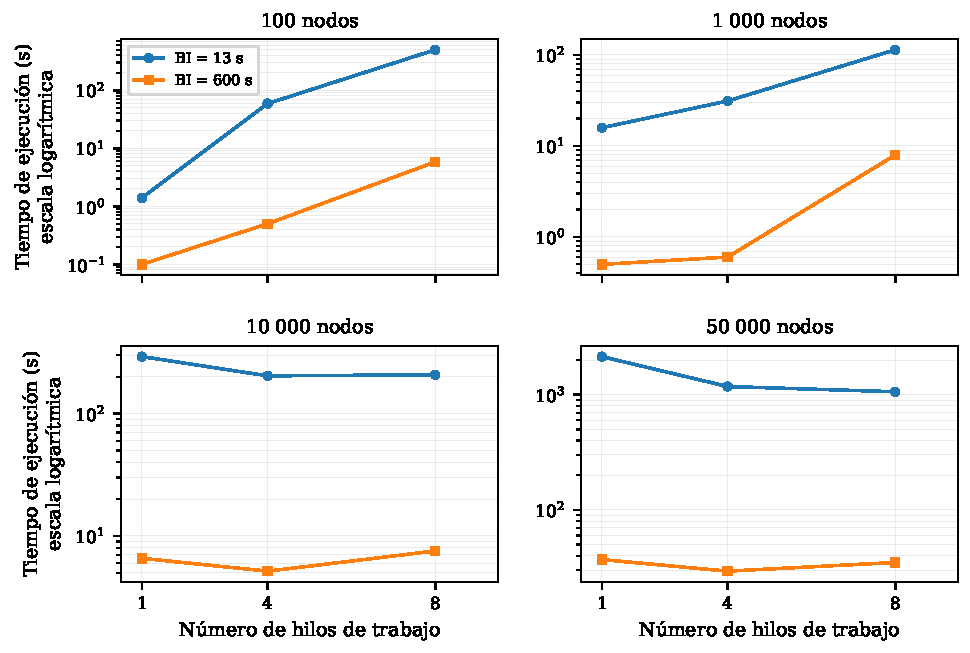
\includegraphics[width=\textwidth]{figures/fig_performance.pdf}
  \caption{Tiempos de ejecución reproducidos para 1, 4 y 8 hilos de trabajo. Solo se muestran las configuraciones que finalizaron correctamente en la máquina de 12 vCPU. El eje vertical es logarítmico.}
  \label{fig:performance}
\end{figure}

\begin{table}[H]
\caption{Tiempos reproducidos y speedup respecto de un hilo (solo configuraciones válidas).}
\label{tab:performance}
\centering
\footnotesize
\setlength{\tabcolsep}{4pt}
\renewcommand{\arraystretch}{1.12}
\begin{tabular}{lcccccc}
\toprule
\rowcolor{tablehead}
\textbf{Nodos} & \textbf{BI (s)} &
\textbf{$T(1)$ (s)} & \textbf{$T(4)$ (s)} & \textbf{$T(8)$ (s)} &
\textbf{$S(4)$} & \textbf{$S(8)$} \\
\midrule
100     & 13  & 1.400    & 58.837   & 496.974  & 0.02 & 0.003 \\
100     & 600 & 0.100    & 0.501    & 5.810    & 0.20 & 0.017 \\
1\,000  & 13  & 15.874   & 31.176   & 113.962  & 0.51 & 0.14 \\
1\,000  & 600 & 0.500    & 0.601    & 7.937    & 0.83 & 0.06 \\
10\,000 & 13  & 292.029  & 203.329  & 207.492  & 1.44 & 1.41 \\
10\,000 & 600 & 6.564    & 5.155    & 7.543    & 1.27 & 0.87 \\
50\,000 & 13  & 2\,146.348 & 1\,179.811 & 1\,062.808 & 1.82 & 2.02 \\
50\,000 & 600 & 37.028   & 29.354   & 34.949   & 1.26 & 1.06 \\
\bottomrule
\end{tabular}
\end{table}

La degradación en redes pequeñas es el resultado más llamativo. Para 100 nodos y 13\,s, el tiempo pasa de 1.4\,s con un hilo a 58.8\,s con cuatro y a 497.0\,s con ocho, es decir, un speedup de 0.02 y 0.003, respectivamente. Para 1\,000 nodos y 13\,s, el tiempo pasa de 15.9\,s a 31.2\,s y 114.0\,s. Este comportamiento es consistente con la explicación del artículo: cuando el número de hilos se acerca al número de LPs, el sesgo de reloj y las cascadas de rollback dominan el costo de la sincronización. Sin embargo, la magnitud observada es mucho mayor que la reportada.

La Figura~\ref{fig:performance_vs_paper} compara los tiempos reproducidos con los del artículo en los hilos comunes (1, 4 y 8). En la red de 100 nodos, el artículo reporta una mejora moderada (12.4\,s a 7.3\,s y 6.7\,s para 13\,s), mientras que la reproducción muestra una degradación severa. En 1\,000 y 10\,000 nodos, el artículo reporta speedups de 2.5--4.5$\times$ a 8 hilos; la reproducción obtiene 1.4$\times$ en 10\,000 nodos y 0.14$\times$ en 1\,000 nodos. Los tiempos absolutos de un hilo son, sin embargo, mucho menores en la reproducción: 15.9\,s frente a 392.1\,s en 1\,000 nodos y 292.0\,s frente a 5\,966.0\,s en 10\,000 nodos.

\begin{figure}[H]
  \centering
  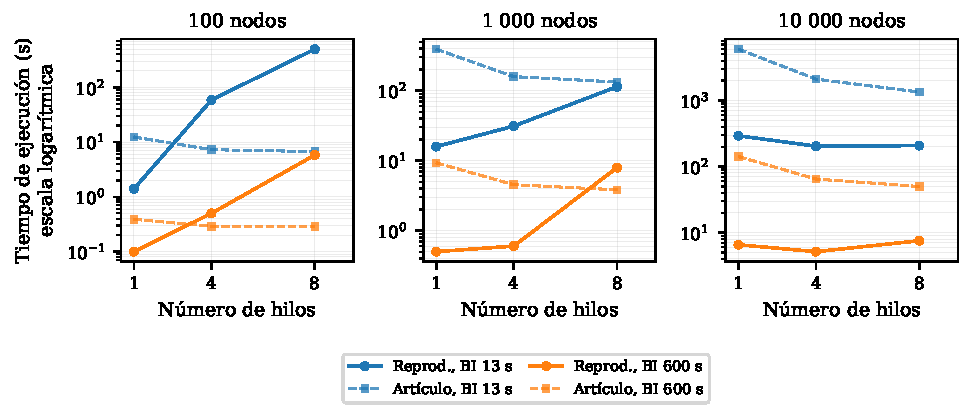
\includegraphics[width=\textwidth]{figures/fig_performance_vs_paper.pdf}
  \caption{Comparación de tiempos reproducidos (líneas continuas) con los valores digitalizados del artículo (líneas discontinuas) en los hilos comunes 1, 4 y 8. El eje vertical es logarítmico. Los valores del artículo provienen de la Figura~6 y se usan como referencia aproximada.}
  \label{fig:performance_vs_paper}
\end{figure}

La Tabla~\ref{tab:comparacion_rendimiento} presenta la comparación numérica. La relación artículo/reproducción en un hilo varía entre 3.9 y 24.7; en 4 y 8 hilos la relación se invierte en las redes pequeñas, donde la reproducción es más lenta. Para 50\,000 nodos no existe un valor directo en el artículo; la comparación con 100\,000 nodos muestra que la reproducción es entre 20 y 65 veces más rápida, pero la diferencia de tamaño de red impide una comparación directa.

\begin{table}[H]
\caption{Comparación de tiempos con el artículo en los hilos comunes (valores del artículo digitalizados de la Figura~6).}
\label{tab:comparacion_rendimiento}
\centering
\footnotesize
\setlength{\tabcolsep}{3pt}
\renewcommand{\arraystretch}{1.10}
\begin{tabular}{lcccccccc}
\toprule
\rowcolor{tablehead}
\textbf{Nodos} & \textbf{BI} &
\textbf{Art. 1} & \textbf{Rep. 1} &
\textbf{Art. 4} & \textbf{Rep. 4} &
\textbf{Art. 8} & \textbf{Rep. 8} \\
\midrule
100     & 13  & 12.4     & 1.400    & 7.26     & 58.837   & 6.71     & 496.974 \\
100     & 600 & 0.39     & 0.100    & 0.29     & 0.501    & 0.29     & 5.810 \\
1\,000  & 13  & 392.06   & 15.874   & 158.63   & 31.176   & 132.95   & 113.962 \\
1\,000  & 600 & 9.30     & 0.500    & 4.53     & 0.601    & 3.82     & 7.937 \\
10\,000 & 13  & 5\,965.97 & 292.029 & 2\,102.57 & 203.329 & 1\,339.27 & 207.492 \\
10\,000 & 600 & 141.56   & 6.564    & 64.66    & 5.155    & 49.81    & 7.543 \\
50\,000 & 13  & ---      & 2\,146.348 & ---    & 1\,179.811 & ---    & 1\,062.808 \\
50\,000 & 600 & ---      & 37.028   & ---      & 29.354   & ---      & 34.949 \\
\bottomrule
\end{tabular}
\end{table}

\subsection{Uso de memoria}

La Figura~\ref{fig:ram} muestra la RAM máxima reproducida para 1, 4 y 8 hilos, y la Tabla~\ref{tab:ram} la compara con los valores aproximados del artículo. Para 10\,000 nodos, la reproducción obtiene 3.5--5.0\,GB, en línea con el rango de 3.4--5.9\,GB que se desprende de la Figura~7 del artículo. Para 50\,000 nodos, la reproducción obtiene 16.6--24.9\,GB; el artículo no reporta 50\,000 nodos, pero sus valores para 100\,000 nodos (35--47\,GB en la Figura~7) son consistentes con un crecimiento aproximadamente lineal.

\begin{figure}[H]
  \centering
  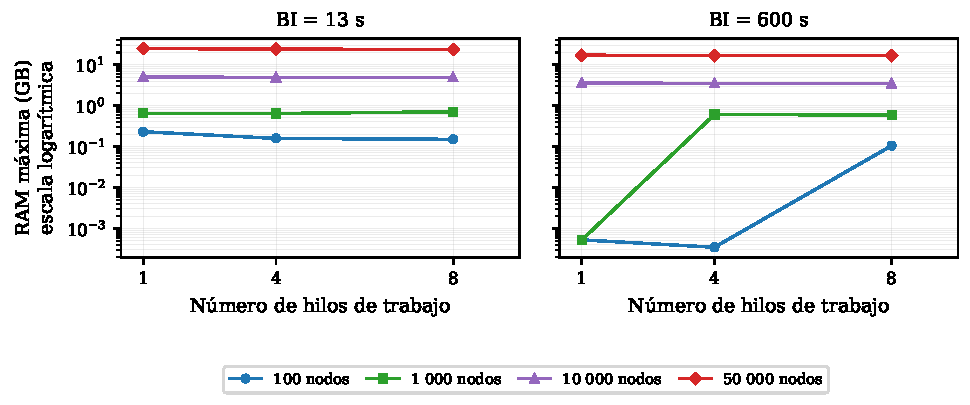
\includegraphics[width=\textwidth]{figures/fig_ram.pdf}
  \caption{RAM máxima reproducida para 1, 4 y 8 hilos. Solo se incluyen configuraciones válidas. El eje vertical es logarítmico. Los valores inferiores a 0.01\,GB corresponden a ejecuciones muy cortas y deben interpretarse con cautela.}
  \label{fig:ram}
\end{figure}

\begin{table}[H]
\caption{RAM máxima reproducida y comparación aproximada con la Figura~7 del artículo.}
\label{tab:ram}
\centering
\footnotesize
\setlength{\tabcolsep}{4pt}
\renewcommand{\arraystretch}{1.12}
\begin{tabular}{lcccc}
\toprule
\rowcolor{tablehead}
\textbf{Nodos} & \textbf{BI} &
\textbf{Reprod. 1/4/8 hilos (GB)} &
\textbf{Artículo (GB, aprox.)} &
\textbf{Observación} \\
\midrule
100     & 13  & 0.23 / 0.16 / 0.15 & $\sim$0.4--0.5 & Reproducción menor \\
100     & 600 & 0.0005 / 0.0004 / 0.105 & $\sim$0.3--0.5 & Valores no representativos \\
1\,000  & 13  & 0.65 / 0.64 / 0.71 & $\sim$0.4 / 0.9 / 1.3 & Reproducción menor \\
1\,000  & 600 & 0.001 / 0.606 / 0.592 & $\sim$0.2 / 0.3 / 0.4 & Valores bajos con 1 hilo \\
10\,000 & 13  & 5.03 / 4.89 / 4.92 & $\sim$3.5 / 4.4 / 4.8 & Coincidencia razonable \\
10\,000 & 600 & 3.56 / 3.50 / 3.47 & $\sim$3.4 / 3.5 / 3.6 & Coincidencia alta \\
50\,000 & 13  & 24.9 / 24.1 / 23.5 & 100k: $\sim$35--47 & Consistente con 50k \\
50\,000 & 600 & 17.1 / 16.7 / 16.6 & 100k: $\sim$33--40 & Consistente con 50k \\
\bottomrule
\end{tabular}
\end{table}

Los valores anómalamente bajos de 100 nodos con 600\,s y de 1\,000 nodos con 600\,s y un hilo se explican por la duración extremadamente corta de esas ejecuciones (0.1\,s y 0.5\,s): el muestreador de memoria no alcanza a registrar el pico real. Por esa razón, la comparación de memoria se apoya principalmente en las redes de 10\,000 y 50\,000 nodos, cuyas ejecuciones duran decenas o cientos de segundos.

La Figura~\ref{fig:ram_history} muestra la evolución agregada de la memoria durante la simulación para 1\,000, 10\,000 y 50\,000 nodos. La memoria crece rápidamente al inicio, se estabiliza y permanece acotada hasta el final. Los valores de meseta son aproximadamente 0.6\,GB para 1\,000 nodos, 3.5\,GB para 10\,000 y 16.5\,GB para 50\,000. La tendencia y la forma de las curvas son cualitativamente similares a las de la Figura~8 del artículo, aunque los valores absolutos son menores: el artículo muestra aproximadamente 1\,GB para 1\,000 nodos, 8--9\,GB para 10\,000 y 35\,GB para 100\,000.

\begin{figure}[H]
  \centering
  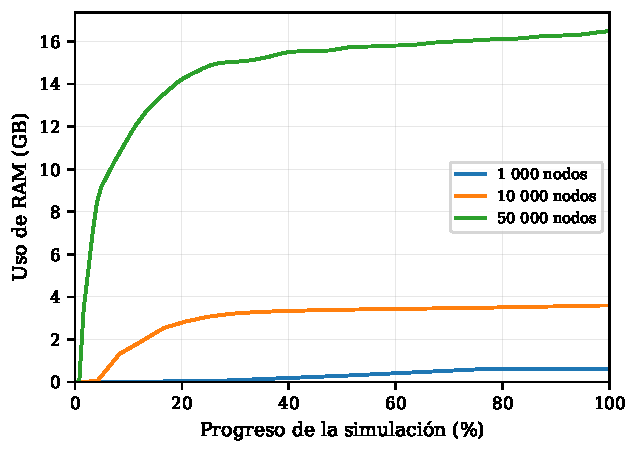
\includegraphics[width=0.78\textwidth]{figures/fig_ram_history.pdf}
  \caption{Evolución agregada del uso de RAM durante la simulación para 1\,000, 10\,000 y 50\,000 nodos (equivalente a la Figura~8 del artículo).}
  \label{fig:ram_history}
\end{figure}

\subsection{Resumen de la reproducción}

La Tabla~\ref{tab:resumen} sintetiza el estado de cada figura. La reproducibilidad es alta para la validación estadística y los ataques, parcial para la memoria y baja para el rendimiento en el rango de hilos disponible. Las casillas marcadas como ``no verificable'' no implican un fallo del artículo, sino la imposibilidad de ejecutar la configuración correspondiente en la máquina utilizada.

\begin{table}[H]
\caption{Resumen del estado de reproducción de las figuras del artículo.}
\label{tab:resumen}
\centering
\small
\renewcommand{\arraystretch}{1.15}
\begin{tabularx}{\textwidth}{lXXl}
\toprule
\rowcolor{tablehead}
\textbf{Figura} & \textbf{Artículo} & \textbf{Reproducción} & \textbf{Estado} \\
\midrule
3 & Tasa de minería proporcional a la potencia de hash & $R^2 \ge 0.9969$, MAE $\le 0.0127$ & Conforme \\
4a--4c & 51\,\% sigue la diagonal & MAE 0.020--0.031 & Conforme \\
4d--4f & Minería egoísta; profundidad 3 compromete menos & Tendencias equivalentes & Conforme (cualitativo) \\
5 & Éxito crece con $h$ y se satura & Curvas equivalentes, más irregulares & Conforme (cualitativo) \\
6 & Pico de rendimiento en 16--22 hilos & Solo 1/4/8 hilos; sin pico verificable & Parcial / no verificable \\
7 & 10k: 3.4--5.9\,GB; 100k: 35--47\,GB & 10k: 3.5--5.0\,GB; 50k: 16.6--24.9\,GB & Conforme en orden de magnitud \\
8 & 1k: $\sim$1\,GB; 10k: 8--9\,GB; 100k: $\sim$35\,GB & 1k: 0.6\,GB; 10k: 3.5\,GB; 50k: 16.5\,GB & Parcial \\
\bottomrule
\end{tabularx}
\end{table}

%============================================================
%  5. COMPARACIÓN CON EL ARTÍCULO
%============================================================
\section{Comparación con el artículo}
\label{sec:comparacion}

\subsection{Validación estadística y ataques}

La comparación de la Figura~3 es satisfactoria. El artículo afirma que la tasa observada sigue la esperada y que el modelo respeta la proporcionalidad estadística; la reproducción lo confirma cuantitativamente con $R^2$ superior a 0.9969 y MAE inferior a 1.3 puntos porcentuales. La reproducibilidad es especialmente alta en 1\,000 nodos, donde el MAE es 0.0086.

En el ataque del 51\,\%, el artículo concluye que poseer una mayor potencia de hash sin sabotear activamente la red no produce una aceptación desproporcionada de bloques, incluso con un nodo obstinado que favorece ramas donde minó más. La reproducción respalda esa conclusión: las curvas de ambas tolerancias se mantienen cerca de la diagonal y los errores son inferiores a 10 puntos porcentuales. La principal diferencia es la rugosidad: el artículo promedia cinco ejecuciones y la reproducción usa una sola, por lo que los puntos individuales tienen mayor varianza.

En la minería egoísta, el artículo observa que el ataque puede tener éxito incluso con una fracción modesta de la potencia de hash, pero que sin al menos el 50\,\% es contraproducente en términos de bloques comprometidos. La reproducción reproduce ambas tendencias: la tasa de éxito crece con $h$ y se satura, mientras que el porcentaje comprometido de las configuraciones de profundidad 3 se sitúa por debajo de la diagonal en potencias bajas y medias. Las diferencias numéricas son mayores que en el 51\,\%, especialmente en la forma de las curvas, pero la dirección y el orden de magnitud son consistentes.

\subsection{Rendimiento}

La comparación de rendimiento es la parte menos concluyente. El artículo reporta que el rendimiento mejora al aumentar los hilos y alcanza un máximo en 16--22 hilos, para luego degradarse. En la reproducción no fue posible ejecutar 16 o más hilos, por lo que el pico no puede verificarse. En el rango 1--8 hilos, el artículo muestra speedups en todas las redes; la reproducción muestra speedups solo en 10\,000 y 50\,000 nodos, y una degradación severa en 100 y 1\,000 nodos.

Esta discrepancia puede deberse a varios factores. Primero, el artículo utilizó una máquina con 44 núcleos físicos y 88 hyperthreads, mientras que la reproducción dispuso de 6 núcleos físicos y 12 hyperthreads. Segundo, el artículo promedia cinco ejecuciones, mientras que la reproducción ejecutó una sola; aunque esto no cambia el tiempo medio por ejecución, sí afecta la estabilidad de las mediciones y la posibilidad de descartar valores atípicos. Tercero, el artefacto no registra en los metadatos la topología efectiva ni el fanout utilizado; el \texttt{entrypoint.py} invoca \texttt{generate\_topology.py} con 2--6 vecinos, mientras que la topología por defecto del repositorio usa 40--120 vecinos. Esta ambigüedad puede alterar el número de eventos y el costo de los rollbacks. Cuarto, los tiempos absolutos de un hilo son entre 4 y 25 veces menores en la reproducción, lo que sugiere diferencias de build, de versión del código o de carga de la máquina que no pueden aislarse con los datos disponibles.

Un cálculo sencillo muestra que, si los valores del artículo se interpretaran como la suma de cinco ejecuciones en lugar de su promedio, la diferencia en un hilo se reduciría a un factor de 4--5, más compatible con la diferencia de arquitectura. El artículo afirma explícitamente que los valores son promedios, por lo que esta hipótesis no puede confirmarse; se menciona solo como una posible explicación de la magnitud de la discrepancia. En cualquier caso, la comparación de tiempos absolutos entre hardware distinto no es una prueba de incorrectitud del artículo, sino una limitación del entorno de reproducción.

\subsection{Uso de memoria}

La comparación de memoria es más favorable. Para 10\,000 nodos, la reproducción obtiene 3.5--5.0\,GB, dentro del rango aproximado de 3.4--5.9\,GB de la Figura~7 del artículo. Para 50\,000 nodos, la reproducción obtiene 16.6--24.9\,GB, consistente con un crecimiento aproximadamente lineal desde los 35--47\,GB reportados para 100\,000 nodos. La Figura~8 reproducida muestra la misma forma de crecimiento y estabilización que la del artículo, con valores absolutos menores en 1\,000 y 10\,000 nodos.

Existe una inconsistencia en el artículo entre el texto y la Figura~7: el texto afirma que para 100\,000 nodos se observó un pico de 99.8\,GB, mientras que la Figura~7 muestra valores cercanos a 35--47\,GB. La reproducción no permite resolver esta inconsistencia porque la red más grande fue de 50\,000 nodos. Se deja constancia de ella como un aspecto que merece aclaración por parte de los autores.

\subsection{Síntesis}

En conjunto, la reproducción confirma la corrección funcional y estadística de RBlockSim y la validez cualitativa de sus resultados de ataques. La reproducibilidad de rendimiento es limitada por el hardware y por la imposibilidad de ejecutar los hilos altos; la reproducibilidad de memoria es buena en orden de magnitud. La Tabla~\ref{tab:resumen} resume esta evaluación.

%============================================================
%  6. DISCUSIÓN Y LIMITACIONES
%============================================================
\section{Discusión y limitaciones}
\label{sec:discusion}

\subsection{Interpretación de los resultados}

Los resultados de validación estadística y de ataques son los más robustos porque dependen de la lógica del modelo y no del tiempo de ejecución. La alta correlación entre potencia de hash y tasa de minería indica que el generador de bloques respeta la distribución de Poisson y que la asignación de potencia se implementa correctamente. El ataque del 51\,\% sigue la diagonal, lo que sugiere que el mecanismo de consenso no favorece artificialmente al atacante. La minería egoísta reproduce el comportamiento esperado: el éxito aumenta con la potencia de hash, la profundidad 3 es más costosa en términos de bloques comprometidos y la saturación se alcanza para potencias altas.

La degradación del rendimiento en redes pequeñas es coherente con la teoría de PDES. Con 100 nodos y 8 hilos, hay menos de 13 LPs por hilo; el sesgo de reloj y las cascadas de rollback pueden superar ampliamente el beneficio del paralelismo. El artículo menciona este efecto y limita la Figura~6a a 16 hilos, pero la magnitud observada en la reproducción es mayor. Es posible que la topología utilizada en la reproducción tenga una densidad diferente a la del artículo, o que el build y la versión del runtime respondan de forma distinta en un procesador con menos núcleos.

\subsection{Limitaciones}

Las limitaciones principales de este trabajo son las siguientes.

\begin{enumerate}
  \item \textbf{Límite de núcleos.} La máquina dispone de 12 vCPU. Las ejecuciones con 16, 22, 44, 66 y 88 hilos fallaron, por lo que no se pudo verificar el pico de rendimiento en 16--22 hilos ni la degradación posterior. Los resultados de rendimiento se limitan a 1, 4 y 8 hilos.
  \item \textbf{Una sola iteración.} El artículo promedia cinco ejecuciones en la mayoría de los casos; la reproducción ejecutó una sola iteración por configuración. Esto aumenta la varianza de las curvas de ataque y de los tiempos, y explica en parte la rugosidad de las Figuras~4 y~5.
  \item \textbf{Red más grande reducida.} La red de 100\,000 nodos se sustituyó por 50\,000 nodos por limitaciones de memoria y tiempo. La comparación con la Figura~6d y con la Figura~8 del artículo es, por tanto, indirecta.
  \item \textbf{Hardware distinto.} El procesador, la memoria y el número de núcleos difieren del servidor del artículo. Los tiempos absolutos no son directamente comparables; solo lo son las tendencias y los speedups.
  \item \textbf{Configuración no registrada.} El artefacto no guarda en los metadatos la topología efectiva, el fanout ni otros parámetros de red. \texttt{entrypoint.py} invoca 2--6 vecinos, mientras que la topología por defecto del repositorio usa 40--120. Esta ambigüedad impide atribuir con certeza las diferencias de rendimiento.
  \item \textbf{Figuras del artículo digitalizadas.} Los valores de las Figuras~6 y~7 del artículo se obtuvieron por digitalización visual del PDF, no de una tabla de datos. Son aproximados y se usan solo como referencia.
  \item \textbf{Sin ejecución distribuida.} No se probó el modo MPI ni la ejecución en varias máquinas, que el artículo menciona como una ventaja para redes muy grandes.
\end{enumerate}

\subsection{Amenazas a la validez}

La validez interna de los resultados de ataques está limitada por el uso de una sola semilla por configuración. Aunque las semillas son aleatorias y los resultados agregados son estables, no se calcularon intervalos de confianza ni pruebas de significancia. La validez externa está limitada por el tamaño de red y por la topología: los resultados de 100, 1\,000 y 10\,000 nodos no necesariamente se generalizan a redes de 100\,000 nodos o a topologías más densas. La validez de constructo de la tasa de éxito de la minería egoísta depende de la definición operativa del trazador original; se mantuvo esa definición para ser consistente con el artículo.

\subsection{Trabajo futuro}

Como trabajo futuro se propone: (i) repetir la campaña en una máquina con al menos 22 núcleos físicos para verificar el pico de 16--22 hilos; (ii) ejecutar cinco iteraciones por configuración para obtener promedios e intervalos de confianza; (iii) reproducir la red de 100\,000 nodos y el modo MPI; (iv) registrar en los metadatos la topología, el fanout y los parámetros de red efectivos; (v) corregir el trazador para que omita las ejecuciones fallidas en lugar de dibujarlas como cero; y (vi) explorar la sensibilidad de los resultados a la densidad de la topología y al fanout.

%============================================================
%  7. CONCLUSIONES
%============================================================
\section{Conclusiones}
\label{sec:conclusiones}

Este trabajo reprodujo el artefacto de RBlockSim y comparó sus resultados con los publicados en SIGSIM-PADS 2025. Las conclusiones principales son las siguientes.

\begin{enumerate}
  \item \textbf{La validación estadística se reproduce con alta fidelidad.} La tasa de minería observada sigue la esperada con $R^2 \ge 0.9969$ y MAE $\le 0.0127$ en las tres redes. El modelo de Proof of Work basado en una distribución exponencial es estadísticamente correcto.
  \item \textbf{Los ataques se reproducen cualitativamente.} El ataque del 51\,\% sigue la diagonal y no muestra una aceptación desproporcionada; la minería egoísta muestra el crecimiento y la saturación esperados, y la profundidad 3 reduce el porcentaje de bloques comprometidos. Las curvas son más irregulares por la ausencia de repeticiones.
  \item \textbf{El rendimiento no se reproduce en el rango disponible.} En 100 y 1\,000 nodos, la paralelización degrada el tiempo; en 10\,000 y 50\,000 nodos, mejora moderadamente. El pico en 16--22 hilos no pudo verificarse por el límite de 12 vCPU. Los tiempos absolutos de un hilo son mucho menores que los del artículo, lo que apunta a diferencias de hardware, build o configuración.
  \item \textbf{La memoria es consistente en orden de magnitud.} Los 10\,000 nodos requieren 3.5--5.0\,GB y los 50\,000 nodos 16.6--24.9\,GB. La tendencia y la forma de las curvas de la Figura~8 son similares a las del artículo, con valores absolutos menores.
  \item \textbf{La reproducibilidad de rendimiento requiere documentar el entorno.} La ausencia de registro de la topología y del fanout, junto con la diferencia de núcleos y el número de iteraciones, impide una comparación concluyente. Una campaña de reproducción debería reportar estos parámetros y ejecutar los hilos altos en hardware adecuado.
\end{enumerate}

En términos globales, RBlockSim demuestra ser un simulador funcionalmente reproducible y estadísticamente sólido. Sus resultados de ataques son robustos y sus resultados de memoria son razonables. La parte de rendimiento es la más sensible al entorno y la que más se beneficiaría de una especificación más detallada de la configuración y de una máquina con más núcleos.

%============================================================
%  REFERENCIAS
%============================================================
\cleardoublepage

\printbibliography[title={Referencias}]

%============================================================
%  APÉNDICE
%============================================================
\appendix
\section{Datos digitalizados del artículo}

Las Tablas~\ref{tab:paper6} y~\ref{tab:paper7} contienen los valores del artículo utilizados en las comparaciones. Fueron digitalizados a partir de las Figuras~6 y~7 del PDF y deben interpretarse como aproximaciones.

\begin{table}[H]
\caption{Valores de la Figura~6 del artículo para todos los hilos reportados (segundos).}
\label{tab:paper6}
\centering
\footnotesize
\setlength{\tabcolsep}{4pt}
\renewcommand{\arraystretch}{1.10}
\begin{tabular}{lccccccc}
\toprule
\rowcolor{tablehead}
\textbf{Nodos} & \textbf{BI} & \textbf{1} & \textbf{4} & \textbf{8} & \textbf{16} & \textbf{22} & \textbf{44} \\
\midrule
100     & 13  & 12.40 & 7.26 & 6.71 & 4.66 & --- & --- \\
100     & 600 & 0.39 & 0.29 & 0.29 & 0.30 & --- & --- \\
1\,000  & 13  & 392.06 & 158.63 & 132.95 & 64.51 & 65.61 & 96.92 \\
1\,000  & 600 & 9.30 & 4.53 & 3.82 & 2.65 & 2.93 & 5.42 \\
10\,000 & 13  & 5\,965.97 & 2\,102.57 & 1\,339.27 & 702.21 & 688.89 & 1\,006.55 \\
10\,000 & 600 & 141.56 & 64.66 & 49.81 & 45.93 & 51.13 & 60.24 \\
100\,000 & 13 & 109\,247.34 & 33\,339.45 & 20\,820.60 & 9\,745.39 & 8\,396.52 & 9\,528.59 \\
100\,000 & 600 & 2\,419.60 & 881.34 & 767.74 & 646.76 & 633.59 & 640.75 \\
\bottomrule
\end{tabular}
\end{table}

\begin{table}[H]
\caption{Valores de la Figura~6 del artículo para 66 y 88 hilos (segundos).}
\label{tab:paper6b}
\centering
\footnotesize
\setlength{\tabcolsep}{5pt}
\renewcommand{\arraystretch}{1.10}
\begin{tabular}{lcccc}
\toprule
\rowcolor{tablehead}
\textbf{Nodos} & \textbf{BI} & \textbf{66} & \textbf{88} \\
\midrule
100     & 13  & --- & --- \\
100     & 600 & --- & --- \\
1\,000  & 13  & 313.25 & 1\,003.83 \\
1\,000  & 600 & 5.98 & 35.16 \\
10\,000 & 13  & 808.41 & 873.93 \\
10\,000 & 600 & 62.06 & 66.02 \\
100\,000 & 13 & 9\,871.87 & 10\,286.61 \\
100\,000 & 600 & 606.04 & 664.93 \\
\bottomrule
\end{tabular}
\end{table}

\begin{table}[H]
\caption{Valores aproximados de la Figura~7 del artículo para 1, 4 y 8 hilos (GB).}
\label{tab:paper7}
\centering
\small
\renewcommand{\arraystretch}{1.15}
\begin{tabular}{lccc}
\toprule
\rowcolor{tablehead}
\textbf{Nodos} & \textbf{1 hilo} & \textbf{4 hilos} & \textbf{8 hilos} \\
\midrule
100     & $\sim$0.3--0.5 & $\sim$0.3--0.5 & $\sim$0.3--0.5 \\
1\,000  & $\sim$0.2--0.4 & $\sim$0.3--0.9 & $\sim$0.4--1.3 \\
10\,000 & $\sim$3.4--3.5 & $\sim$3.5--4.4 & $\sim$3.6--4.8 \\
100\,000 & $\sim$33--36 & $\sim$40--47 & $\sim$38--47 \\
\bottomrule
\end{tabular}
\end{table}

\end{document}
